% -----------------------
\subsection{Dekorationen}
% -----------------------
\begin{minipage}{0.7\textwidth}
  \footnotesize
  % parcolor version 2011-09-30
\begingroup
\ttfamily
\definecolor{R}{named}{Red}
\definecolor{G}{named}{ForestGreen}
\definecolor{B}{named}{RoyalBlue}
\definecolor{C}{named}{Cyan}
\definecolor{M}{named}{Magenta}
\definecolor{Y}{named}{YellowOrange}
\definecolor{background}{rgb}{0.82, 0.82, 0.92}
\dimen255=\textwidth
\advance\dimen255 by -2\fboxsep
\noindent
\colorbox{background}
{%
\parbox{\dimen255}
{%
\rule[-0.5ex]{0pt}{2.5ex}\hspace*{0.0em}\textcolor{G}{\textbf{\%~benoetigt~\textbackslash{}usetikzlibrary\{decorations.pathmorphing\}}}\\
\rule[-0.5ex]{0pt}{2.5ex}\hspace*{0.0em}\textbackslash{}draw[\textcolor{R}{\textbf{decorate}},~\textcolor{R}{\textbf{decoration=bent}}]~(0,~0)~{-}{-}~(3,~0);}%
}%
\endgroup

\end{minipage}\hfill
\begin{minipage}{0.29\textwidth}
  \centering
  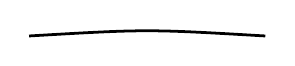
\begin{tikzpicture}[line width=1pt]
    % benoetigt \usetikzlibrary{decorations.pathmorphing}
    \draw[decorate, decoration=bent] (0, 0) -- (3, 0);
  \end{tikzpicture}
\end{minipage}

\begin{minipage}{0.7\textwidth}
  \footnotesize
  % parcolor version 2011-09-30
\begingroup
\ttfamily
\definecolor{R}{named}{Red}
\definecolor{G}{named}{ForestGreen}
\definecolor{B}{named}{RoyalBlue}
\definecolor{C}{named}{Cyan}
\definecolor{M}{named}{Magenta}
\definecolor{Y}{named}{YellowOrange}
\definecolor{background}{rgb}{0.82, 0.82, 0.92}
\dimen255=\textwidth
\advance\dimen255 by -2\fboxsep
\noindent
\colorbox{background}
{%
\parbox{\dimen255}
{%
\rule[-0.5ex]{0pt}{2.5ex}\hspace*{0.0em}\textcolor{G}{\textbf{\%~benoetigt~\textbackslash{}usetikzlibrary\{decorations.pathmorphing\}}}\\
\rule[-0.5ex]{0pt}{2.5ex}\hspace*{0.0em}\textbackslash{}draw[\textcolor{R}{\textbf{decorate}},~\textcolor{R}{\textbf{decoration=bumps}}]~(0,~0)~{-}{-}~(3,~0);}%
}%
\endgroup

\end{minipage}\hfill
\begin{minipage}{0.29\textwidth}
  \centering
  
\begin{tikzpicture}[line width=1pt]
    % benoetigt \usetikzlibrary{decorations.pathmorphing}
    \draw[decorate, decoration=bumps] (0, 0) -- (3, 0);
  \end{tikzpicture}
\end{minipage}

\begin{minipage}{0.7\textwidth}
  \footnotesize
  % parcolor version 2011-09-30
\begingroup
\ttfamily
\definecolor{R}{named}{Red}
\definecolor{G}{named}{ForestGreen}
\definecolor{B}{named}{RoyalBlue}
\definecolor{C}{named}{Cyan}
\definecolor{M}{named}{Magenta}
\definecolor{Y}{named}{YellowOrange}
\definecolor{background}{rgb}{0.82, 0.82, 0.92}
\dimen255=\textwidth
\advance\dimen255 by -2\fboxsep
\noindent
\colorbox{background}
{%
\parbox{\dimen255}
{%
\rule[-0.5ex]{0pt}{2.5ex}\hspace*{0.0em}\textcolor{G}{\textbf{\%~benoetigt~\textbackslash{}usetikzlibrary\{decorations.pathmorphing\}}}\\
\rule[-0.5ex]{0pt}{2.5ex}\hspace*{0.0em}\textbackslash{}draw[\textcolor{R}{\textbf{decorate}},~\textcolor{R}{\textbf{decoration=coil}}]~(0,~0)~{-}{-}~(3,~0);}%
}%
\endgroup

\end{minipage}\hfill
\begin{minipage}{0.29\textwidth}
  \centering
  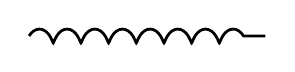
\begin{tikzpicture}[line width=1pt]
    % benoetigt \usetikzlibrary{decorations.pathmorphing}
    \draw[decorate, decoration=coil] (0, 0) -- (3, 0);
  \end{tikzpicture}
\end{minipage}

\begin{minipage}{0.7\textwidth}
  \footnotesize
  % parcolor version 2011-09-30
\begingroup
\ttfamily
\definecolor{R}{named}{Red}
\definecolor{G}{named}{ForestGreen}
\definecolor{B}{named}{RoyalBlue}
\definecolor{C}{named}{Cyan}
\definecolor{M}{named}{Magenta}
\definecolor{Y}{named}{YellowOrange}
\definecolor{background}{rgb}{0.82, 0.82, 0.92}
\dimen255=\textwidth
\advance\dimen255 by -2\fboxsep
\noindent
\colorbox{background}
{%
\parbox{\dimen255}
{%
\rule[-0.5ex]{0pt}{2.5ex}\hspace*{0.0em}\textcolor{G}{\textbf{\%~benoetigt~\textbackslash{}usetikzlibrary\{decorations.pathmorphing\}}}\\
\rule[-0.5ex]{0pt}{2.5ex}\hspace*{0.0em}\textbackslash{}draw[\textcolor{R}{\textbf{decorate}},~\textcolor{R}{\textbf{decoration=random~steps}}]~(0,~0)~{-}{-}~(3,~0);}%
}%
\endgroup

\end{minipage}\hfill
\begin{minipage}{0.29\textwidth}
  \centering
  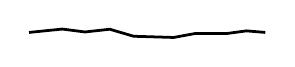
\begin{tikzpicture}[line width=1pt]
    % benoetigt \usetikzlibrary{decorations.pathmorphing}
    \draw[decorate, decoration=random steps] (0, 0) -- (3, 0);
  \end{tikzpicture}
\end{minipage}

\begin{minipage}{0.7\textwidth}
  \footnotesize
  % parcolor version 2011-09-30
\begingroup
\ttfamily
\definecolor{R}{named}{Red}
\definecolor{G}{named}{ForestGreen}
\definecolor{B}{named}{RoyalBlue}
\definecolor{C}{named}{Cyan}
\definecolor{M}{named}{Magenta}
\definecolor{Y}{named}{YellowOrange}
\definecolor{background}{rgb}{0.82, 0.82, 0.92}
\dimen255=\textwidth
\advance\dimen255 by -2\fboxsep
\noindent
\colorbox{background}
{%
\parbox{\dimen255}
{%
\rule[-0.5ex]{0pt}{2.5ex}\hspace*{0.0em}\textcolor{G}{\textbf{\%~benoetigt~\textbackslash{}usetikzlibrary\{decorations.pathmorphing\}}}\\
\rule[-0.5ex]{0pt}{2.5ex}\hspace*{0.0em}\textbackslash{}draw[\textcolor{R}{\textbf{decorate}},~\textcolor{R}{\textbf{decoration=saw}}]~(0,~0)~{-}{-}~(3,~0);}%
}%
\endgroup

\end{minipage}\hfill
\begin{minipage}{0.29\textwidth}
  \centering
  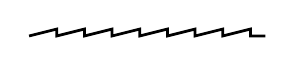
\begin{tikzpicture}[line width=1pt]
    % benoetigt \usetikzlibrary{decorations.pathmorphing}
    \draw[decorate, decoration=saw] (0, 0) -- (3, 0);
  \end{tikzpicture}
\end{minipage}

\begin{minipage}{0.7\textwidth}
  \footnotesize
  % parcolor version 2011-09-30
\begingroup
\ttfamily
\definecolor{R}{named}{Red}
\definecolor{G}{named}{ForestGreen}
\definecolor{B}{named}{RoyalBlue}
\definecolor{C}{named}{Cyan}
\definecolor{M}{named}{Magenta}
\definecolor{Y}{named}{YellowOrange}
\definecolor{background}{rgb}{0.82, 0.82, 0.92}
\dimen255=\textwidth
\advance\dimen255 by -2\fboxsep
\noindent
\colorbox{background}
{%
\parbox{\dimen255}
{%
\rule[-0.5ex]{0pt}{2.5ex}\hspace*{0.0em}\textcolor{G}{\textbf{\%~benoetigt~\textbackslash{}usetikzlibrary\{decorations.pathmorphing\}}}\\
\rule[-0.5ex]{0pt}{2.5ex}\hspace*{0.0em}\textbackslash{}draw[\textcolor{R}{\textbf{decorate}},~\textcolor{R}{\textbf{decoration=snake}}]~(0,~0)~{-}{-}~(3,~0);}%
}%
\endgroup

\end{minipage}\hfill
\begin{minipage}{0.29\textwidth}
  \centering
  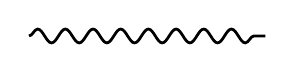
\begin{tikzpicture}[line width=1pt]
    % benoetigt \usetikzlibrary{decorations.pathmorphing}
    \draw[decorate, decoration=snake] (0, 0) -- (3, 0);
  \end{tikzpicture}
\end{minipage}

\begin{minipage}{0.7\textwidth}
  \footnotesize
  % parcolor version 2011-09-30
\begingroup
\ttfamily
\definecolor{R}{named}{Red}
\definecolor{G}{named}{ForestGreen}
\definecolor{B}{named}{RoyalBlue}
\definecolor{C}{named}{Cyan}
\definecolor{M}{named}{Magenta}
\definecolor{Y}{named}{YellowOrange}
\definecolor{background}{rgb}{0.82, 0.82, 0.92}
\dimen255=\textwidth
\advance\dimen255 by -2\fboxsep
\noindent
\colorbox{background}
{%
\parbox{\dimen255}
{%
\rule[-0.5ex]{0pt}{2.5ex}\hspace*{0.0em}\textcolor{G}{\textbf{\%~benoetigt~\textbackslash{}usetikzlibrary\{decorations.pathmorphing\}}}\\
\rule[-0.5ex]{0pt}{2.5ex}\hspace*{0.0em}\textbackslash{}draw[\textcolor{R}{\textbf{decorate}},~\textcolor{R}{\textbf{decoration=zigzag}}]~(0,~0)~{-}{-}~(3,~0);}%
}%
\endgroup

\end{minipage}\hfill
\begin{minipage}{0.29\textwidth}
  \centering
  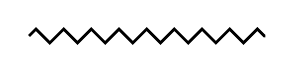
\begin{tikzpicture}[line width=1pt]
    % benoetigt \usetikzlibrary{decorations.pathmorphing}
    \draw[decorate, decoration=zigzag] (0, 0) -- (3, 0);
  \end{tikzpicture}
\end{minipage}

\begin{minipage}{0.7\textwidth}
  \footnotesize
  % parcolor version 2011-09-30
\begingroup
\ttfamily
\definecolor{R}{named}{Red}
\definecolor{G}{named}{ForestGreen}
\definecolor{B}{named}{RoyalBlue}
\definecolor{C}{named}{Cyan}
\definecolor{M}{named}{Magenta}
\definecolor{Y}{named}{YellowOrange}
\definecolor{background}{rgb}{0.82, 0.82, 0.92}
\dimen255=\textwidth
\advance\dimen255 by -2\fboxsep
\noindent
\colorbox{background}
{%
\parbox{\dimen255}
{%
\rule[-0.5ex]{0pt}{2.5ex}\hspace*{0.0em}\textcolor{G}{\textbf{\%~benoetigt~\textbackslash{}usetikzlibrary\{decorations.pathreplacing\}}}\\
\rule[-0.5ex]{0pt}{2.5ex}\hspace*{0.0em}\textbackslash{}draw[\textcolor{R}{\textbf{decorate}},~\textcolor{R}{\textbf{decoration=border}}]~(0,~0)~{-}{-}~(3,~0);}%
}%
\endgroup

\end{minipage}\hfill
\begin{minipage}{0.29\textwidth}
  \centering
  \begin{tikzpicture}[line width=1pt]
    % benoetigt \usetikzlibrary{decorations.pathreplacing}
    \draw[decorate, decoration=border] (0, 0) -- (3, 0);
  \end{tikzpicture}
\end{minipage}

\begin{minipage}{0.7\textwidth}
  \footnotesize
  % parcolor version 2011-09-30
\begingroup
\ttfamily
\definecolor{R}{named}{Red}
\definecolor{G}{named}{ForestGreen}
\definecolor{B}{named}{RoyalBlue}
\definecolor{C}{named}{Cyan}
\definecolor{M}{named}{Magenta}
\definecolor{Y}{named}{YellowOrange}
\definecolor{background}{rgb}{0.82, 0.82, 0.92}
\dimen255=\textwidth
\advance\dimen255 by -2\fboxsep
\noindent
\colorbox{background}
{%
\parbox{\dimen255}
{%
\rule[-0.5ex]{0pt}{2.5ex}\hspace*{0.0em}\textcolor{G}{\textbf{\%~benoetigt~\textbackslash{}usetikzlibrary\{decorations.pathreplacing\}}}\\
\rule[-0.5ex]{0pt}{2.5ex}\hspace*{0.0em}\textbackslash{}draw[\textcolor{R}{\textbf{decorate}},~\textcolor{R}{\textbf{decoration=brace}}]~(0,~0)~{-}{-}~(3,~0);}%
}%
\endgroup

\end{minipage}\hfill
\begin{minipage}{0.29\textwidth}
  \centering
  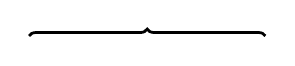
\begin{tikzpicture}[line width=1pt]
    % benoetigt \usetikzlibrary{decorations.pathreplacing}
    \draw[decorate, decoration=brace] (0, 0) -- (3, 0);
  \end{tikzpicture}
\end{minipage}

\begin{minipage}{0.7\textwidth}
  \footnotesize
  % parcolor version 2011-09-30
\begingroup
\ttfamily
\definecolor{R}{named}{Red}
\definecolor{G}{named}{ForestGreen}
\definecolor{B}{named}{RoyalBlue}
\definecolor{C}{named}{Cyan}
\definecolor{M}{named}{Magenta}
\definecolor{Y}{named}{YellowOrange}
\definecolor{background}{rgb}{0.82, 0.82, 0.92}
\dimen255=\textwidth
\advance\dimen255 by -2\fboxsep
\noindent
\colorbox{background}
{%
\parbox{\dimen255}
{%
\rule[-0.5ex]{0pt}{2.5ex}\hspace*{0.0em}\textcolor{G}{\textbf{\%~benoetigt~\textbackslash{}usetikzlibrary\{decorations.pathreplacing\}}}\\
\rule[-0.5ex]{0pt}{2.5ex}\hspace*{0.0em}\textbackslash{}draw[\textcolor{R}{\textbf{decorate}},~\textcolor{R}{\textbf{decoration}}=\{\textcolor{R}{\textbf{expanding~waves}},~angle=10\}]\\
\rule[-0.5ex]{0pt}{2.5ex}\hspace*{2.5em}(0,~0)~{-}{-}~(3,~0);}%
}%
\endgroup

\end{minipage}\hfill
\begin{minipage}{0.29\textwidth}
  \centering
  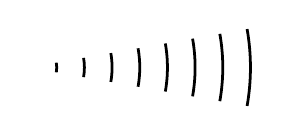
\begin{tikzpicture}[line width=1pt]
    % benoetigt \usetikzlibrary{decorations.pathreplacing}
    \draw[decorate, decoration={expanding waves, angle=10}]
         (0, 0) -- (3, 0);
  \end{tikzpicture}
\end{minipage}

\begin{minipage}{0.7\textwidth}
  \footnotesize
  % parcolor version 2011-09-30
\begingroup
\ttfamily
\definecolor{R}{named}{Red}
\definecolor{G}{named}{ForestGreen}
\definecolor{B}{named}{RoyalBlue}
\definecolor{C}{named}{Cyan}
\definecolor{M}{named}{Magenta}
\definecolor{Y}{named}{YellowOrange}
\definecolor{background}{rgb}{0.82, 0.82, 0.92}
\dimen255=\textwidth
\advance\dimen255 by -2\fboxsep
\noindent
\colorbox{background}
{%
\parbox{\dimen255}
{%
\rule[-0.5ex]{0pt}{2.5ex}\hspace*{0.0em}\textcolor{G}{\textbf{\%~benoetigt~\textbackslash{}usetikzlibrary\{decorations.pathreplacing\}}}\\
\rule[-0.5ex]{0pt}{2.5ex}\hspace*{0.0em}\textbackslash{}draw[\textcolor{R}{\textbf{decorate}},~\textcolor{R}{\textbf{decoration=ticks}}]~(0,~0)~{-}{-}~(3,~0);}%
}%
\endgroup

\end{minipage}\hfill
\begin{minipage}{0.29\textwidth}
  \centering
  \begin{tikzpicture}[line width=1pt]
    % benoetigt \usetikzlibrary{decorations.pathreplacing}
    \draw[decorate, decoration=ticks] (0, 0) -- (3, 0);
  \end{tikzpicture}
\end{minipage}

\begin{minipage}{0.7\textwidth}
  \footnotesize
  % parcolor version 2011-09-30
\begingroup
\ttfamily
\definecolor{R}{named}{Red}
\definecolor{G}{named}{ForestGreen}
\definecolor{B}{named}{RoyalBlue}
\definecolor{C}{named}{Cyan}
\definecolor{M}{named}{Magenta}
\definecolor{Y}{named}{YellowOrange}
\definecolor{background}{rgb}{0.82, 0.82, 0.92}
\dimen255=\textwidth
\advance\dimen255 by -2\fboxsep
\noindent
\colorbox{background}
{%
\parbox{\dimen255}
{%
\rule[-0.5ex]{0pt}{2.5ex}\hspace*{0.0em}\textcolor{G}{\textbf{\%~benoetigt~\textbackslash{}usetikzlibrary\{decorations.pathreplacing\}}}\\
\rule[-0.5ex]{0pt}{2.5ex}\hspace*{0.0em}\textbackslash{}draw[\textcolor{R}{\textbf{decorate}},~\textcolor{R}{\textbf{decoration=waves}}]~(0,~0)~{-}{-}~(3,~0);}%
}%
\endgroup

\end{minipage}\hfill
\begin{minipage}{0.29\textwidth}
  \centering
  \begin{tikzpicture}[line width=1pt]
    % benoetigt \usetikzlibrary{decorations.pathreplacing}
    \draw[decorate, decoration=waves] (0, 0) -- (3, 0);
  \end{tikzpicture}
\end{minipage}

\begin{minipage}{0.7\textwidth}
  \footnotesize
  % parcolor version 2011-09-30
\begingroup
\ttfamily
\definecolor{R}{named}{Red}
\definecolor{G}{named}{ForestGreen}
\definecolor{B}{named}{RoyalBlue}
\definecolor{C}{named}{Cyan}
\definecolor{M}{named}{Magenta}
\definecolor{Y}{named}{YellowOrange}
\definecolor{background}{rgb}{0.82, 0.82, 0.92}
\dimen255=\textwidth
\advance\dimen255 by -2\fboxsep
\noindent
\colorbox{background}
{%
\parbox{\dimen255}
{%
\rule[-0.5ex]{0pt}{2.5ex}\hspace*{0.0em}\textcolor{G}{\textbf{\%~benoetigt~\textbackslash{}usetikzlibrary\{decorations.shapes\}}}\\
\rule[-0.5ex]{0pt}{2.5ex}\hspace*{0.0em}\textbackslash{}draw[\textcolor{R}{\textbf{decorate}},~\textcolor{R}{\textbf{decoration=crosses}}]~(0,~0)~{-}{-}~(3,~0);}%
}%
\endgroup

\end{minipage}\hfill
\begin{minipage}{0.29\textwidth}
  \centering
  \begin{tikzpicture}[line width=1pt]
    % benoetigt \usetikzlibrary{decorations.shapes}
    \draw[decorate, decoration=crosses] (0, 0) -- (3, 0);
  \end{tikzpicture}
\end{minipage}

\begin{minipage}{0.7\textwidth}
  \footnotesize
  % parcolor version 2011-09-30
\begingroup
\ttfamily
\definecolor{R}{named}{Red}
\definecolor{G}{named}{ForestGreen}
\definecolor{B}{named}{RoyalBlue}
\definecolor{C}{named}{Cyan}
\definecolor{M}{named}{Magenta}
\definecolor{Y}{named}{YellowOrange}
\definecolor{background}{rgb}{0.82, 0.82, 0.92}
\dimen255=\textwidth
\advance\dimen255 by -2\fboxsep
\noindent
\colorbox{background}
{%
\parbox{\dimen255}
{%
\rule[-0.5ex]{0pt}{2.5ex}\hspace*{0.0em}\textcolor{G}{\textbf{\%~benoetigt~\textbackslash{}usetikzlibrary\{decorations.shapes\}}}\\
\rule[-0.5ex]{0pt}{2.5ex}\hspace*{0.0em}\textbackslash{}draw[\textcolor{R}{\textbf{decorate}},~\textcolor{R}{\textbf{decoration=shape~backgrounds}}]\\
\rule[-0.5ex]{0pt}{2.5ex}\hspace*{2.5em}(0,~0)~{-}{-}~(3,~0);}%
}%
\endgroup

\end{minipage}\hfill
\begin{minipage}{0.29\textwidth}
  \centering
  \begin{tikzpicture}[line width=1pt]
    % benoetigt \usetikzlibrary{decorations.shapes}
    \draw[decorate, decoration=shape backgrounds]
         (0, 0) -- (3, 0);
  \end{tikzpicture}
\end{minipage}

\begin{minipage}{0.7\textwidth}
  \footnotesize
  % parcolor version 2011-09-30
\begingroup
\ttfamily
\definecolor{R}{named}{Red}
\definecolor{G}{named}{ForestGreen}
\definecolor{B}{named}{RoyalBlue}
\definecolor{C}{named}{Cyan}
\definecolor{M}{named}{Magenta}
\definecolor{Y}{named}{YellowOrange}
\definecolor{background}{rgb}{0.82, 0.82, 0.92}
\dimen255=\textwidth
\advance\dimen255 by -2\fboxsep
\noindent
\colorbox{background}
{%
\parbox{\dimen255}
{%
\rule[-0.5ex]{0pt}{2.5ex}\hspace*{0.0em}\textcolor{G}{\textbf{\%~benoetigt~\textbackslash{}usetikzlibrary\{decorations.shapes\}}}\\
\rule[-0.5ex]{0pt}{2.5ex}\hspace*{0.0em}\textbackslash{}draw[\textcolor{R}{\textbf{decorate}},~\textcolor{R}{\textbf{decoration=triangles}}]~(0,~0)~{-}{-}~(3,~0);}%
}%
\endgroup

\end{minipage}\hfill
\begin{minipage}{0.29\textwidth}
  \centering
  \begin{tikzpicture}[line width=1pt]
    % benoetigt \usetikzlibrary{decorations.shapes}
    \draw[decorate, decoration=triangles] (0, 0) -- (3, 0);
  \end{tikzpicture}
\end{minipage}

\begin{minipage}{0.7\textwidth}
  \footnotesize
  % parcolor version 2011-09-30
\begingroup
\ttfamily
\definecolor{R}{named}{Red}
\definecolor{G}{named}{ForestGreen}
\definecolor{B}{named}{RoyalBlue}
\definecolor{C}{named}{Cyan}
\definecolor{M}{named}{Magenta}
\definecolor{Y}{named}{YellowOrange}
\definecolor{background}{rgb}{0.82, 0.82, 0.92}
\dimen255=\textwidth
\advance\dimen255 by -2\fboxsep
\noindent
\colorbox{background}
{%
\parbox{\dimen255}
{%
\rule[-0.5ex]{0pt}{2.5ex}\hspace*{0.0em}\textcolor{G}{\textbf{\%~benoetigt~\textbackslash{}usetikzlibrary\{decorations.text\}}}\\
\rule[-0.5ex]{0pt}{2.5ex}\hspace*{0.0em}\textbackslash{}draw[\textcolor{R}{\textbf{decorate}},~\textcolor{R}{\textbf{decoration}}=\{\textcolor{R}{\textbf{text~along~path}},\\
\rule[-0.5ex]{0pt}{2.5ex}\hspace*{14.0em}\textcolor{R}{\textbf{text=\{abcdefghijklmnopqr\}}}\}]\\
\rule[-0.5ex]{0pt}{2.5ex}\hspace*{2.5em}(0,~0)~..~controls~(1,~2)~and~(1,~0)~..~(3,~0);}%
}%
\endgroup

\end{minipage}\hfill
\begin{minipage}{0.29\textwidth}
  \centering
  \begin{tikzpicture}
    \clip (-3mm, -1mm) rectangle (28mm, 13mm);
    % benoetigt \usetikzlibrary{decorations.text}
    \draw[decorate, decoration={text along path,
                                text={abcdefghijklmnopqr}}]
         (0, 0) .. controls (1, 2) and (1, 0) .. (3, 0);
  \end{tikzpicture}
\end{minipage}

